% REV01 Thu 24 Jun 2021 06:34:15 WIB
% START Tue 04 May 2021 13:55:16 WIB

\chapter{THE SAME RESPECTED FRIEND IN MORE ASPECTS THAN ONE}

In sooth, it is Riderhood and no other, or it is the outer husk and
shell of Riderhood and no other, that is borne into Miss Abbey’s
first-floor bedroom. Supple to twist and turn as the Rogue has ever
been, he is sufficiently rigid now; and not without much shuffling of
attendant feet, and tilting of his bier this way and that way, and
peril even of his sliding off it and being tumbled in a heap over the
balustrades, can he be got up stairs.

‘Fetch a doctor,’ quoth Miss Abbey. And then, ‘Fetch his daughter.’ On
both of which errands, quick messengers depart.

The doctor-seeking messenger meets the doctor halfway, coming under
convoy of police. Doctor examines the dank carcase, and pronounces, not
hopefully, that it is worth while trying to reanimate the same. All the
best means are at once in action, and everybody present lends a hand,
and a heart and soul. No one has the least regard for the man; with them
all, he has been an object of avoidance, suspicion, and aversion; but
the spark of life within him is curiously separable from himself now,
and they have a deep interest in it, probably because it IS life, and
they are living and must die.

In answer to the doctor’s inquiry how did it happen, and was anyone to
blame, Tom Tootle gives in his verdict, unavoidable accident and no one
to blame but the sufferer. ‘He was slinking about in his boat,’ says
Tom, ‘which slinking were, not to speak ill of the dead, the manner of
the man, when he come right athwart the steamer’s bows and she cut him
in two.’ Mr Tootle is so far figurative, touching the dismemberment, as
that he means the boat, and not the man. For, the man lies whole before
them.

Captain Joey, the bottle-nosed regular customer in the glazed hat, is a
pupil of the much-respected old school, and (having insinuated himself
into the chamber, in the execution of the important service of carrying
the drowned man’s neck-kerchief) favours the doctor with a sagacious
old-scholastic suggestion that the body should be hung up by the heels,
‘sim’lar’, says Captain Joey, ‘to mutton in a butcher’s shop,’ and
should then, as a particularly choice manoeuvre for promoting easy
respiration, be rolled upon casks. These scraps of the wisdom of the
captain’s ancestors are received with such speechless indignation by
Miss Abbey, that she instantly seizes the Captain by the collar, and
without a single word ejects him, not presuming to remonstrate, from the
scene.

There then remain, to assist the doctor and Tom, only those three other
regular customers, Bob Glamour, William Williams, and Jonathan (family
name of the latter, if any, unknown to man-kind), who are quite enough.
Miss Abbey having looked in to make sure that nothing is wanted,
descends to the bar, and there awaits the result, with the gentle Jew
and Miss Jenny Wren.

If you are not gone for good, Mr Riderhood, it would be something to
know where you are hiding at present. This flabby lump of mortality that
we work so hard at with such patient perseverance, yields no sign of
you. If you are gone for good, Rogue, it is very solemn, and if you are
coming back, it is hardly less so. Nay, in the suspense and mystery of
the latter question, involving that of where you may be now, there is a
solemnity even added to that of death, making us who are in attendance
alike afraid to look on you and to look off you, and making those below
start at the least sound of a creaking plank in the floor.

Stay! Did that eyelid tremble? So the doctor, breathing low, and closely
watching, asks himself.

No.

Did that nostril twitch?

No.

This artificial respiration ceasing, do I feel any faint flutter under
my hand upon the chest?

No.

Over and over again No. No. But try over and over again, nevertheless.

See! A token of life! An indubitable token of life! The spark may
smoulder and go out, or it may glow and expand, but see! The four
rough fellows, seeing, shed tears. Neither Riderhood in this world, nor
Riderhood in the other, could draw tears from them; but a striving human
soul between the two can do it easily.

He is struggling to come back. Now, he is almost here, now he is far
away again. Now he is struggling harder to get back. And yet--like us
all, when we swoon--like us all, every day of our lives when we wake--he
is instinctively unwilling to be restored to the consciousness of this
existence, and would be left dormant, if he could.

Bob Gliddery returns with Pleasant Riderhood, who was out when sought
for, and hard to find. She has a shawl over her head, and her first
action, when she takes it off weeping, and curtseys to Miss Abbey, is to
wind her hair up.

‘Thank you, Miss Abbey, for having father here.’

‘I am bound to say, girl, I didn’t know who it was,’ returns Miss Abbey;
‘but I hope it would have been pretty much the same if I had known.’

Poor Pleasant, fortified with a sip of brandy, is ushered into the
first-floor chamber. She could not express much sentiment about her
father if she were called upon to pronounce his funeral oration, but she
has a greater tenderness for him than he ever had for her, and crying
bitterly when she sees him stretched unconscious, asks the doctor, with
clasped hands: ‘Is there no hope, sir? O poor father! Is poor father
dead?’

To which the doctor, on one knee beside the body, busy and watchful,
only rejoins without looking round: ‘Now, my girl, unless you have the
self-command to be perfectly quiet, I cannot allow you to remain in the
room.’

Pleasant, consequently, wipes her eyes with her back-hair, which is in
fresh need of being wound up, and having got it out of the way, watches
with terrified interest all that goes on. Her natural woman’s aptitude
soon renders her able to give a little help. Anticipating the doctor’s
want of this or that, she quietly has it ready for him, and so by
degrees is intrusted with the charge of supporting her father’s head
upon her arm.

It is something so new to Pleasant to see her father an object of
sympathy and interest, to find any one very willing to tolerate his
society in this world, not to say pressingly and soothingly entreating
him to belong to it, that it gives her a sensation she never experienced
before. Some hazy idea that if affairs could remain thus for a long time
it would be a respectable change, floats in her mind. Also some vague
idea that the old evil is drowned out of him, and that if he should
happily come back to resume his occupation of the empty form that lies
upon the bed, his spirit will be altered. In which state of mind she
kisses the stony lips, and quite believes that the impassive hand she
chafes will revive a tender hand, if it revive ever.

Sweet delusion for Pleasant Riderhood. But they minister to him with
such extraordinary interest, their anxiety is so keen, their vigilance
is so great, their excited joy grows so intense as the signs of life
strengthen, that how can she resist it, poor thing! And now he begins
to breathe naturally, and he stirs, and the doctor declares him to have
come back from that inexplicable journey where he stopped on the dark
road, and to be here.

Tom Tootle, who is nearest to the doctor when he says this, grasps
the doctor fervently by the hand. Bob Glamour, William Williams, and
Jonathan of the no surname, all shake hands with one another round, and
with the doctor too. Bob Glamour blows his nose, and Jonathan of the
no surname is moved to do likewise, but lacking a pocket handkerchief
abandons that outlet for his emotion. Pleasant sheds tears deserving her
own name, and her sweet delusion is at its height.

There is intelligence in his eyes. He wants to ask a question. He
wonders where he is. Tell him.

‘Father, you were run down on the river, and are at Miss Abbey
Potterson’s.’

He stares at his daughter, stares all around him, closes his eyes, and
lies slumbering on her arm.

The short-lived delusion begins to fade. The low, bad, unimpressible
face is coming up from the depths of the river, or what other depths, to
the surface again. As he grows warm, the doctor and the four men cool.
As his lineaments soften with life, their faces and their hearts harden
to him.

‘He will do now,’ says the doctor, washing his hands, and looking at the
patient with growing disfavour.

‘Many a better man,’ moralizes Tom Tootle with a gloomy shake of the
head, ‘ain’t had his luck.’

‘It’s to be hoped he’ll make a better use of his life,’ says Bob
Glamour, ‘than I expect he will.’

‘Or than he done afore,’ adds William Williams.

‘But no, not he!’ says Jonathan of the no surname, clinching the
quartette.

They speak in a low tone because of his daughter, but she sees that they
have all drawn off, and that they stand in a group at the other end of
the room, shunning him. It would be too much to suspect them of being
sorry that he didn’t die when he had done so much towards it, but they
clearly wish that they had had a better subject to bestow their pains
on. Intelligence is conveyed to Miss Abbey in the bar, who reappears on
the scene, and contemplates from a distance, holding whispered discourse
with the doctor. The spark of life was deeply interesting while it was
in abeyance, but now that it has got established in Mr Riderhood, there
appears to be a general desire that circumstances had admitted of its
being developed in anybody else, rather than that gentleman.

‘However,’ says Miss Abbey, cheering them up, ‘you have done your duty
like good and true men, and you had better come down and take something
at the expense of the Porters.’

This they all do, leaving the daughter watching the father. To whom, in
their absence, Bob Gliddery presents himself.

‘His gills looks rum; don’t they?’ says Bob, after inspecting the
patient.

Pleasant faintly nods.

‘His gills’ll look rummer when he wakes; won’t they?’ says Bob.

Pleasant hopes not. Why?

‘When he finds himself here, you know,’ Bob explains. ‘Cause Miss Abbey
forbid him the house and ordered him out of it. But what you may call
the Fates ordered him into it again. Which is rumness; ain’t it?’

‘He wouldn’t have come here of his own accord,’ returns poor Pleasant,
with an effort at a little pride.

‘No,’ retorts Bob. ‘Nor he wouldn’t have been let in, if he had.’

The short delusion is quite dispelled now. As plainly as she sees on her
arm the old father, unimproved, Pleasant sees that everybody there will
cut him when he recovers consciousness. ‘I’ll take him away ever so soon
as I can,’ thinks Pleasant with a sigh; ‘he’s best at home.’

Presently they all return, and wait for him to become conscious that
they will all be glad to get rid of him. Some clothes are got together
for him to wear, his own being saturated with water, and his present
dress being composed of blankets.

Becoming more and more uncomfortable, as though the prevalent dislike
were finding him out somewhere in his sleep and expressing itself to
him, the patient at last opens his eyes wide, and is assisted by his
daughter to sit up in bed.

‘Well, Riderhood,’ says the doctor, ‘how do you feel?’

He replies gruffly, ‘Nothing to boast on.’ Having, in fact, returned to
life in an uncommonly sulky state.

‘I don’t mean to preach; but I hope,’ says the doctor, gravely shaking
his head, ‘that this escape may have a good effect upon you, Riderhood.’

The patient’s discontented growl of a reply is not intelligible; his
daughter, however, could interpret, if she would, that what he says is,
he ‘don’t want no Poll-Parroting’.

Mr Riderhood next demands his shirt; and draws it on over his head (with
his daughter’s help) exactly as if he had just had a Fight.

‘Warn’t it a steamer?’ he pauses to ask her.

‘Yes, father.’

‘I’ll have the law on her, bust her! and make her pay for it.’

He then buttons his linen very moodily, twice or thrice stopping to
examine his arms and hands, as if to see what punishment he has received
in the Fight. He then doggedly demands his other garments, and slowly
gets them on, with an appearance of great malevolence towards his late
opponent and all the spectators. He has an impression that his nose is
bleeding, and several times draws the back of his hand across it, and
looks for the result, in a pugilistic manner, greatly strengthening that
incongruous resemblance.

‘Where’s my fur cap?’ he asks in a surly voice, when he has shuffled his
clothes on.

‘In the river,’ somebody rejoins.\\[2pt]

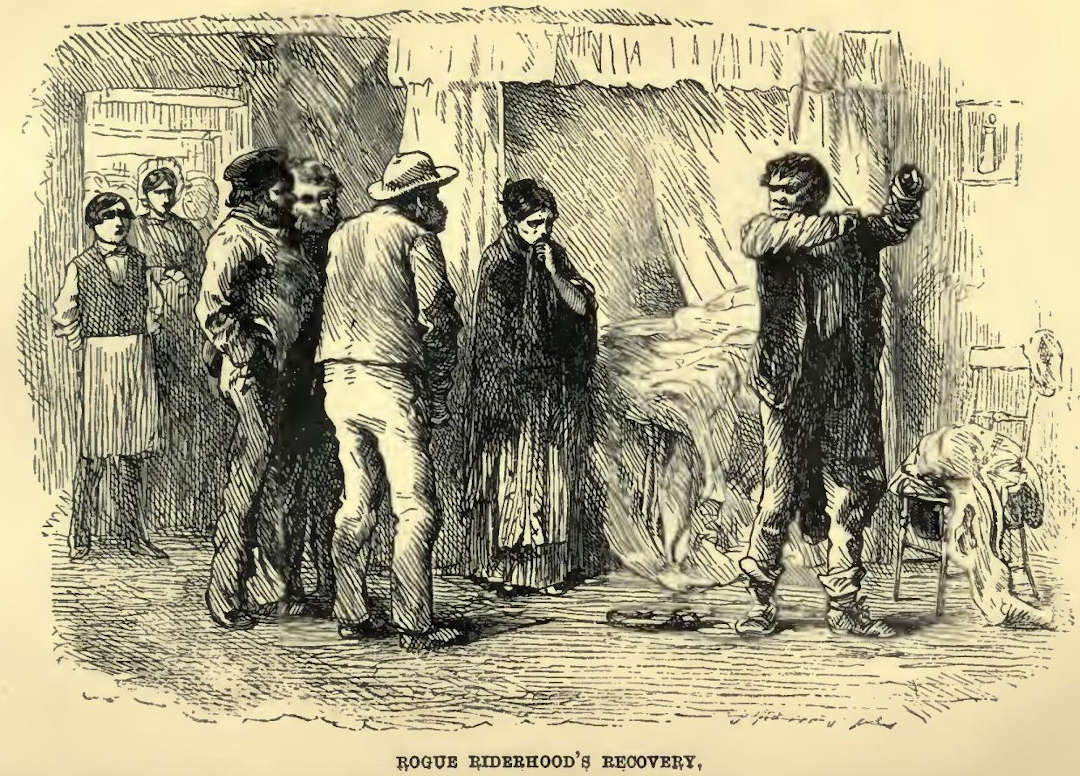
\includegraphics[scale=2.3]{03-03-01}\\[2pt]

‘And warn’t there no honest man to pick it up? O’ course there was
though, and to cut off with it arterwards. You are a rare lot, all on
you!’

Thus, Mr Riderhood: taking from the hands of his daughter, with special
ill-will, a lent cap, and grumbling as he pulls it down over his ears.
Then, getting on his unsteady legs, leaning heavily upon her, and
growling, ‘Hold still, can’t you? What! You must be a staggering next,
must you?’ he takes his departure out of the ring in which he has had
that little turn-up with Death.

